\documentclass[twocolumn,aps,prb,superscriptaddress,longbibliography]{revtex4-2}
%\documentclass[onecolumn,aps,prl,preprint,groupedaddress]{revtex4}
\usepackage{graphicx}
\usepackage{color}
\usepackage{amsmath}
\usepackage[export]{adjustbox}
\usepackage{enumitem}
\usepackage{amssymb}
\usepackage{hyperref}
\usepackage[normalem]{ulem}
\usepackage{adjustbox}
%\usepackage{caption}
%\usepackage{subcaption}

\hypersetup{
	colorlinks = true,
	linkcolor = blue,
	citecolor = blue,
	urlcolor  = blue,
}

\newcommand{\be}{\begin{equation}}
	\newcommand{\ee}{\end{equation}}
\newcommand{\pih}{\frac{2\pi \mathcal{N}}{\hbar}}
\newcommand{\bea}{\begin{eqnarray}}
	\newcommand{\eea}{\end{eqnarray}}
\newcommand{\HH}{{\cal H}}
\newcommand{\RR}{{\cal R}}
\newcommand{\Li}{{\rm Li}}
\newcommand{\p}{\partial}
\newcommand{\s}{\sigma}
\newcommand{\la}{\left\langle}
\newcommand{\ra}{\right\rangle}
\newcommand{\lb}{\left[}
\newcommand{\rb}{\right]}
\newcommand{\lp}{\left(}
\newcommand{\rp}{\right)}
\newcommand{\sgn}{{\rm sgn\,}}
\newcommand{\Tr}{{\rm \, Tr\,}}
\newcommand{\tr}{{\rm \, tr\,}}
\renewcommand{\Re}{{\rm \, Re\,}}
\renewcommand{\Im}{{\rm \, Im\,}}
\newcommand{\sinc}{{\rm \, sinc\,}}
\renewcommand{\vec}[1]{{\boldsymbol #1}}
%\renewcommand{\vec}[1]{{\bf #1}}
\renewcommand{\epsilon}{\varepsilon}
\newcommand{\bra}[1]{\left\langle #1 \right|}
\newcommand{\ket}[1]{\left|#1\right\rangle}
\newcommand{\braket}[2]{\left\langle#1 |  #2\right\rangle}
\newcommand{\braaket}[3]{\left\langle #1 \right| #2 \left|#3 \right\rangle}
\newcommand{\ketbra}[2]{| #1 \rangle\langle #2 |}
\newcommand{\rd}[1]{\mathop{\mathrm{d}#1}}
\newcommand{\tp}[1]{#1^\mathrm{T}}
\newcommand{\hc}[1]{#1^\dagger}
% \renewcommand{\hat}[1]{{\widehat #1}}
\def\nn{\nonumber\\}
\newcommand{\mpar}[1]{\marginpar{\small \it #1}}
\newcommand{\addLL}[1]{\textcolor{red}{#1}}
\newcommand{\addDO}[1]{\textcolor{blue}{#1}}
\newcommand{\addQ}[1]{\textcolor{red}{#1}}
\newcommand{\addmove}[1]{\textcolor{green}{#1}}
\newcommand{\delete}[1]{\textcolor{red}{\sout{#1}}}
\newcommand{\revision}[1]{\textcolor{red}{#1}}
\newcommand{\revisionA}[1]{\textcolor{blue}{#1}}
\newcommand{\revisionB}[1]{\textcolor{magenta}{#1}}
\newcommand{\revisionC}[1]{\textcolor{green}{#1}}
%\renewcommand{\cite}[1]{[\onlinecite{#1}]}

\begin{document}
 \title{Irradiated graphene as a neuromorphic platform}
 
	\date{\today}

    \author{A bunch of friends}
%	\author{D. O. Oriekhov}
	%\affiliation{Kavli Institute of Nanoscience, Delft University of Technology, 2628 CJ Delft, the Netherlands}
	
	\begin{abstract}
		Gapped monolayer graphene is a highly-tunable platform for second harmonic generation in visible and THz frequency light 
		diapason. We show that the nonlinear response of gapped graphene can be used to implement a neuromorphic platform. 
		In particular, we derive the second harmonic response and demonstrate that it implements several computational 
		primitives crucial for modern machine learning computations. Namely, one could view transmitted second harmonic 
		output as a base block of small tensor network, and the combined output with first harmonic - as a nonlinear element 
		of Kolmogorov-Arnold network. We identify the reasonable scales of such device and show the benchmarks in which 
		such device could be efficient compared to electronic analogs. In addition, we demonstrate that graphene shows an 
		important advantage of performing nonlinear transformation of input signal itself. This way one could pass different 
		inputs through the same device.  
	\end{abstract}
	\maketitle

\section{Introduction}

\addDO{Main points to mention:}
\addDO{1: motivation - for main ML approaches, simple nonlinearities are done in GPU's via millions of transistors. Could we instead do photonic low-energy nonlinearities?}

\addDO{2. New approach: light encoding}

\addDO{3. Selection of 2D materials and base effects}

Modern neural-network architectures require vast numbers of multiplications together with repeated applications of nonlinear activation functions to process and propagate data. A significant fraction of this computational overhead is devoted simply to realizing nonlinear maps, even though some convolutional and feature-extraction layers may remain untrained. This motivates a natural question: why not offload part of these demanding operations to physical materials whose intrinsic, unsupervised response already realizes such transformations? Recent studies suggest that this idea is feasible in practice [CITE]. \textcolor{magenta}{in a number of proposed platforms: photonic \cite{Wetzstein2020,Wright2022} [CITE and LIST].} 

\textcolor{magenta}{Among above-mentioned platforms, a special role is taken by linear optical computing. That demonstrates a high energy efficiency and very large input to output conversion sizes, holding high latency even at room temperatures \cite{Yildirim2024,Xia2024,Wang2024NatureCommSc}. The main problem of linearity in optical approaches is resolved by implementing multiple scattering events. That result in nonlinear transformation of scattering potential into output. This method has an advantage of producing separable nonlinearities, but does not leverage the possibility of inputting data via light itself.} Here, we push this direction further by proposing quantum-geometric material nonlinearities as a platform for implementing tensorial data maps directly in matter. 

The Berry phase, the central building block of quantum geometry, plays a foundational role in the modern understanding of electron motion~\cite{RevModPhys.82.1959} and the classification of quantum phases of matter~\cite{RevModPhys.82.3045,RevModPhys.83.1057}. Its associated Berry curvature generates an anomalous contribution to electron velocity and thereby produces the intrinsic Hall effect in systems with broken time-reversal symmetry~\cite{RevModPhys.82.1539}. Strikingly, it has been predicted~\cite{2009arXiv0904.1917D,PhysRevLett.105.026805,PhysRevLett.115.216806} and later observed experimentally~\cite{2018arXiv180908744K,Ma2019,2019arXiv190202699S} that materials with time-reversal symmetry may also host a \textit{nonlinear Hall effect}, controlled by the Berry curvature dipole. Unlike conventional dissipative optical responses, these effects can occur without photon absorption, allowing the material to reshape light while remaining essentially dissipationless. The resulting Kerr and Faraday rotations therefore acquire a tensorial character directly linked to the material’s quantum geometry. This makes quantum-geometric media a natural candidate for implementing optical nonlinear maps.

Two-dimensional materials provide a particularly attractive platform for this program. The 2D materials community already offers a broad range of systems compatible with the architectures considered here, including suspended materials that permit access to both transmission and reflection, as well as heterostructures in which the optical response can be engineered through the top layers. Existing platforms such as MnBi$_2$Te$_4$, MoS$_2$, graphene, twisted graphene, and even their superconducting phases together form a broad and largely unexplored landscape of intrinsic nonlinear responses. In this work, we focus on a few representative examples and show how the Faraday response of a suspended graphene-like material can serve as a functional optical pixel for encoding nonlinear transformations of transmitted light.

\textcolor{magenta}{The obtained nonlinear transformation should be viewed as a computational primitive of machine learning algorithm. We analyze the relevant algorithms based on the encoding of input data into light, by choosing either polarization or amplitudes of components. The input light typically has two polarizations and respective amplitudes, as well as complex phases. Thus, the single layer of quantum-geometric material could produce a polynomial nonlinearity of input vectors in second or higher frequency harmonic. This directly maps to a fixed bond dimension tensor network contraction, a polynomial feature map or a particular case of Kolmogorov-Arnold trainable nonlinearity \cite{liu2024kan20kolmogorovarnoldnetworks}. }

\section{Microscopic model of first- and second-harmonic generation by gapped graphene}

We describe nonlinear optical mapping in thin films through a simple separation of the problem into two subproblems: (i) the microscopic generation of photocurrent in a quantum material driven by a spatially uniform oscillating electric field, and (ii) the self-consistent magneto-optical Maxwell problem for a material layer carrying the current obtained in step (i). This decomposition allows us to connect the intrinsic nonlinear electronic response of the material directly to the emitted and transmitted electromagnetic fields.

This approach has several practical advantages. In the regime of weak oscillating electric fields, screening effects inside the sample can be neglected, since no significant charge buildup is expected when the suspended film is coupled to leads. In alternative architectures, such as heterostructures deposited on a substrate, a similar suppression of screening can be achieved through stronger coupling to an effective bath and sufficiently rapid relaxation. The central object in our treatment is therefore the oscillating photocurrent, with harmonics $\mathbf{j}_{\pm\omega},\mathbf{j}_{\pm2\omega},\mathbf{j}_{\pm3\omega}...$. Because these current components are time-dependent, they do not lead to static charge accumulation, yet they still act as sources of electromagnetic radiation. In the microscopic treatment of the photocurrent, we further neglect effects associated with the magnetic component of the optical field, since these are expected to be parametrically smaller than the electric-field contribution, even up to second and third order in perturbation theory.

\begin{figure}[t]
    \centering
    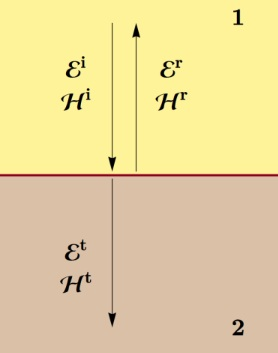
\includegraphics[width=0.2\textwidth]{Figures_for_notes/Kerrs.jpg} % or .pdf, .jpg
    \caption{Illustration for the light scattering on a thin film.}
    \label{fig:1-scattering_field_scheme}
\end{figure}

\subsection{Photocurrent generation}
We now develop a multiband theory applicable to both metals and insulators by incorporating relaxation in the spirit of the relaxation-time approximation. We model the density matrix $\hat\rho$ by the non-Hermitian Liouville equation
\begin{equation}\label{eq01}
    i\hbar\frac{d}{dt}\hat{\rho}(t)-[\hat H_0,\hat\rho(t)]
    =
    -i\hbar\Gamma\big(\hat\rho(t)-\hat\rho^{0}\big),
\end{equation}
where $\Gamma$ is the relaxation rate and $\hat\rho^0$ is the equilibrium density matrix. Standard perturbation theory (see Sec.~B of the Supplementary Information) then yields the photocurrent expansion in terms of the linear and nonlinear conductivity tensors,
\begin{equation}\label{EoM}
    j^\gamma(t)=\int_\omega [\sigma^{(1)}]^{\gamma\beta}_{\omega} E^\beta_{\omega}+\int_{\omega_1,\omega-\omega_1} \hspace{-6mm}[\sigma^{(2)}]^{\gamma\alpha\beta}_{\omega,\omega_1}E^\alpha_{\omega_1}E^\beta_{\omega-\omega_1},
\end{equation}
with $\int_\omega \equiv \int_{-\infty}^{\infty}\frac{d\omega}{2\pi}e^{-i\omega t}$. Although this expression is general, below we specialize to a monochromatic incident drive, $\mathbf E^{\rm i}_\omega=\mathbf E^{\rm i}\delta(\omega-\Omega)+\mathrm{c.c.}$, and to the low-frequency regime $\hbar\Omega\ll\Delta$, where the evolution is adiabatic and essentially non-dissipative.

Importantly, the current is governed by the self-consistent electric field at the film rather than by the bare incident field alone. Therefore, even for a monochromatic drive, the field entering Eq.~(\ref{EoM}) acquires a Floquet harmonic structure through the emitted radiation, $\mathbf E_\omega=\sum_n \mathbf E_n\,\delta(\omega-n\Omega).$ In particular, the generated harmonics are dressed by the linear response of the sheet at the same frequency; for example, the second-harmonic current contains both the nonlinear source term $\hat\sigma^{(2)}_{\Omega,\Omega}:\mathbf E_1\mathbf E_1$ and the linear contribution $\hat\sigma^{(1)}_{2\Omega}\mathbf E_2$. This is the origin of the iterative self-consistent solution described in the next subsection. Here we focus on the photocurrent generation assumed given drive. An important consequence of the self-consistent structure is that the $N$th-order response generically contains a term proportional to $\hat\sigma^{(1)}_{N\Omega}$. Therefore, even if the fundamental drive frequency $\Omega$ lies in the subgap regime, the generated harmonic $N\Omega$ can probe interband physics once it reaches the corresponding excitation threshold.

To suppress interband contributions already at second order, we focus on the optical-gap regime, $\hbar\Omega \ll \Delta_{\rm interband}$, where the response is essentially non-dissipative and no real absorption occurs in the sample, e.g. $\int dt\, \mathbf E(t)\cdot \mathbf j(t)=0$. In this limit, the linear conductivity takes the form
\begin{equation}
    [\hat{\sigma}^{(1)}]^{\gamma \beta}_{\Omega} \hspace{-1mm}=\hspace{-1mm}\frac{e^2}{\hbar}\hspace{-1.5mm}\int_\mathbf{k}\hspace{-0.5mm}\sum_{nm}\hspace{-1mm}\left(\hspace{-1mm}\delta_{nm}\frac{i f_n \partial^\beta_\mathbf{k} \partial^\gamma_\mathbf{k} \epsilon_n}{\hbar\Omega+i\Gamma}\hspace{-0.5mm}-\hspace{-0.5mm}i f_{mn} A^\beta_{nm} A^\gamma_{mn}\hspace{-1mm}\right).
\end{equation}
Here, for a multiband Hamiltonian defined by $\hat H \ket{n,\mathbf{k}} = \epsilon_n(\mathbf{k}) \ket{n,\mathbf{k}}$, the state $\ket{n,\mathbf{k}}$ denotes the periodic part of the Bloch wave function at crystal momentum $\mathbf{k}$. We use $\partial^\alpha_\mathbf{k}\equiv \partial/\partial k^\alpha$, where $(\alpha,\beta,\gamma)$ label Cartesian components. We further define $f_n \equiv f_{\rm FD}[\epsilon_n(\mathbf{k})]$, $f_{nm} \equiv f_n-f_m$, $\epsilon_{nm} \equiv \epsilon_n(\mathbf{k})-\epsilon_m(\mathbf{k})$, and $\mathbf A_{nm}(\mathbf{k}) \equiv \bra{n,\mathbf{k}}\, i\partial_{\mathbf{k}} \,\ket{m,\mathbf{k}}$, with the Fermi-Dirac distribution $f_{\rm FD}(x) \equiv \left(1+\exp\left[{(x-\mu)}/({k_B T})\right]\right)^{-1}$. This expression already reveals several natural tuning knobs, including the chemical potential $\mu$, temperature $T$, and external electrostatic gating. Such controls can strongly modify both the band structure and the associated quantum geometry. Since quantum-geometric effects are often enhanced near band extrema, the resulting optical response is expected to be highly sensitive to both filling and gating. The first term corresponds to the Drude conductivity, while the second describes the linear Hall contribution.

Furthermore, at second order we obtain
\begin{multline}
    [\hat{\sigma}^{(2)}]^{\gamma \alpha \beta}_{\Omega,\Omega}\hspace{-1mm}=\hspace{-1mm}-\frac{e^3}{\hbar}\hspace{-1mm}\int_\mathbf{k}\hspace{-1mm}\sum_{nm}\Bigg\{\frac{\delta_{nm}f_n \partial^\beta_\mathbf{k}\partial^\alpha _\mathbf{k}\partial^\gamma_\mathbf{k}\epsilon_n}{(2\hbar\Omega+i\Gamma)(\hbar\Omega+i\Gamma)}+\\+\frac{A^\gamma_{mn} A^{\alpha }_{nm}\, \partial^\beta_\mathbf{k} f_{mn}}{\hbar\Omega+i\Gamma}\Bigg\},
\end{multline}
The first term corresponds to the jerk nonlinear conductivity, while the second captures the Berry-curvature-dipole (BCD) contribution. To make explicit that the latter is indeed given by the average dipole of the Berry curvature, one may insert a resolution of the identity (see Sec. ? of the Supplementary Information). For simplicity, we focus on the regime $\hbar\Omega \gg \Gamma$. 

The jerk and BCD contributions differ in several important respects. The jerk response is dissipative, whereas the BCD response is Hall-like and dissipationless. Their frequency scaling is also distinct: the jerk contribution scales as $1/\Omega^2$, while the BCD contribution scales as $1/\Omega$. In addition, the jerk response is driven by linearly polarized light, whereas the BCD response is activated by circularly polarized light (see Sec. ? of the Supplementary Information). These differences provide several independent handles for encoding information in the applied electric field and for parametrically distinguishing scattering-sensitive, band-dispersion-controlled currents from those governed by quantum geometry. Most importantly, as we show below, this nonlinear encoding is equivalent to a tensor element.

\begin{figure*}
\centering
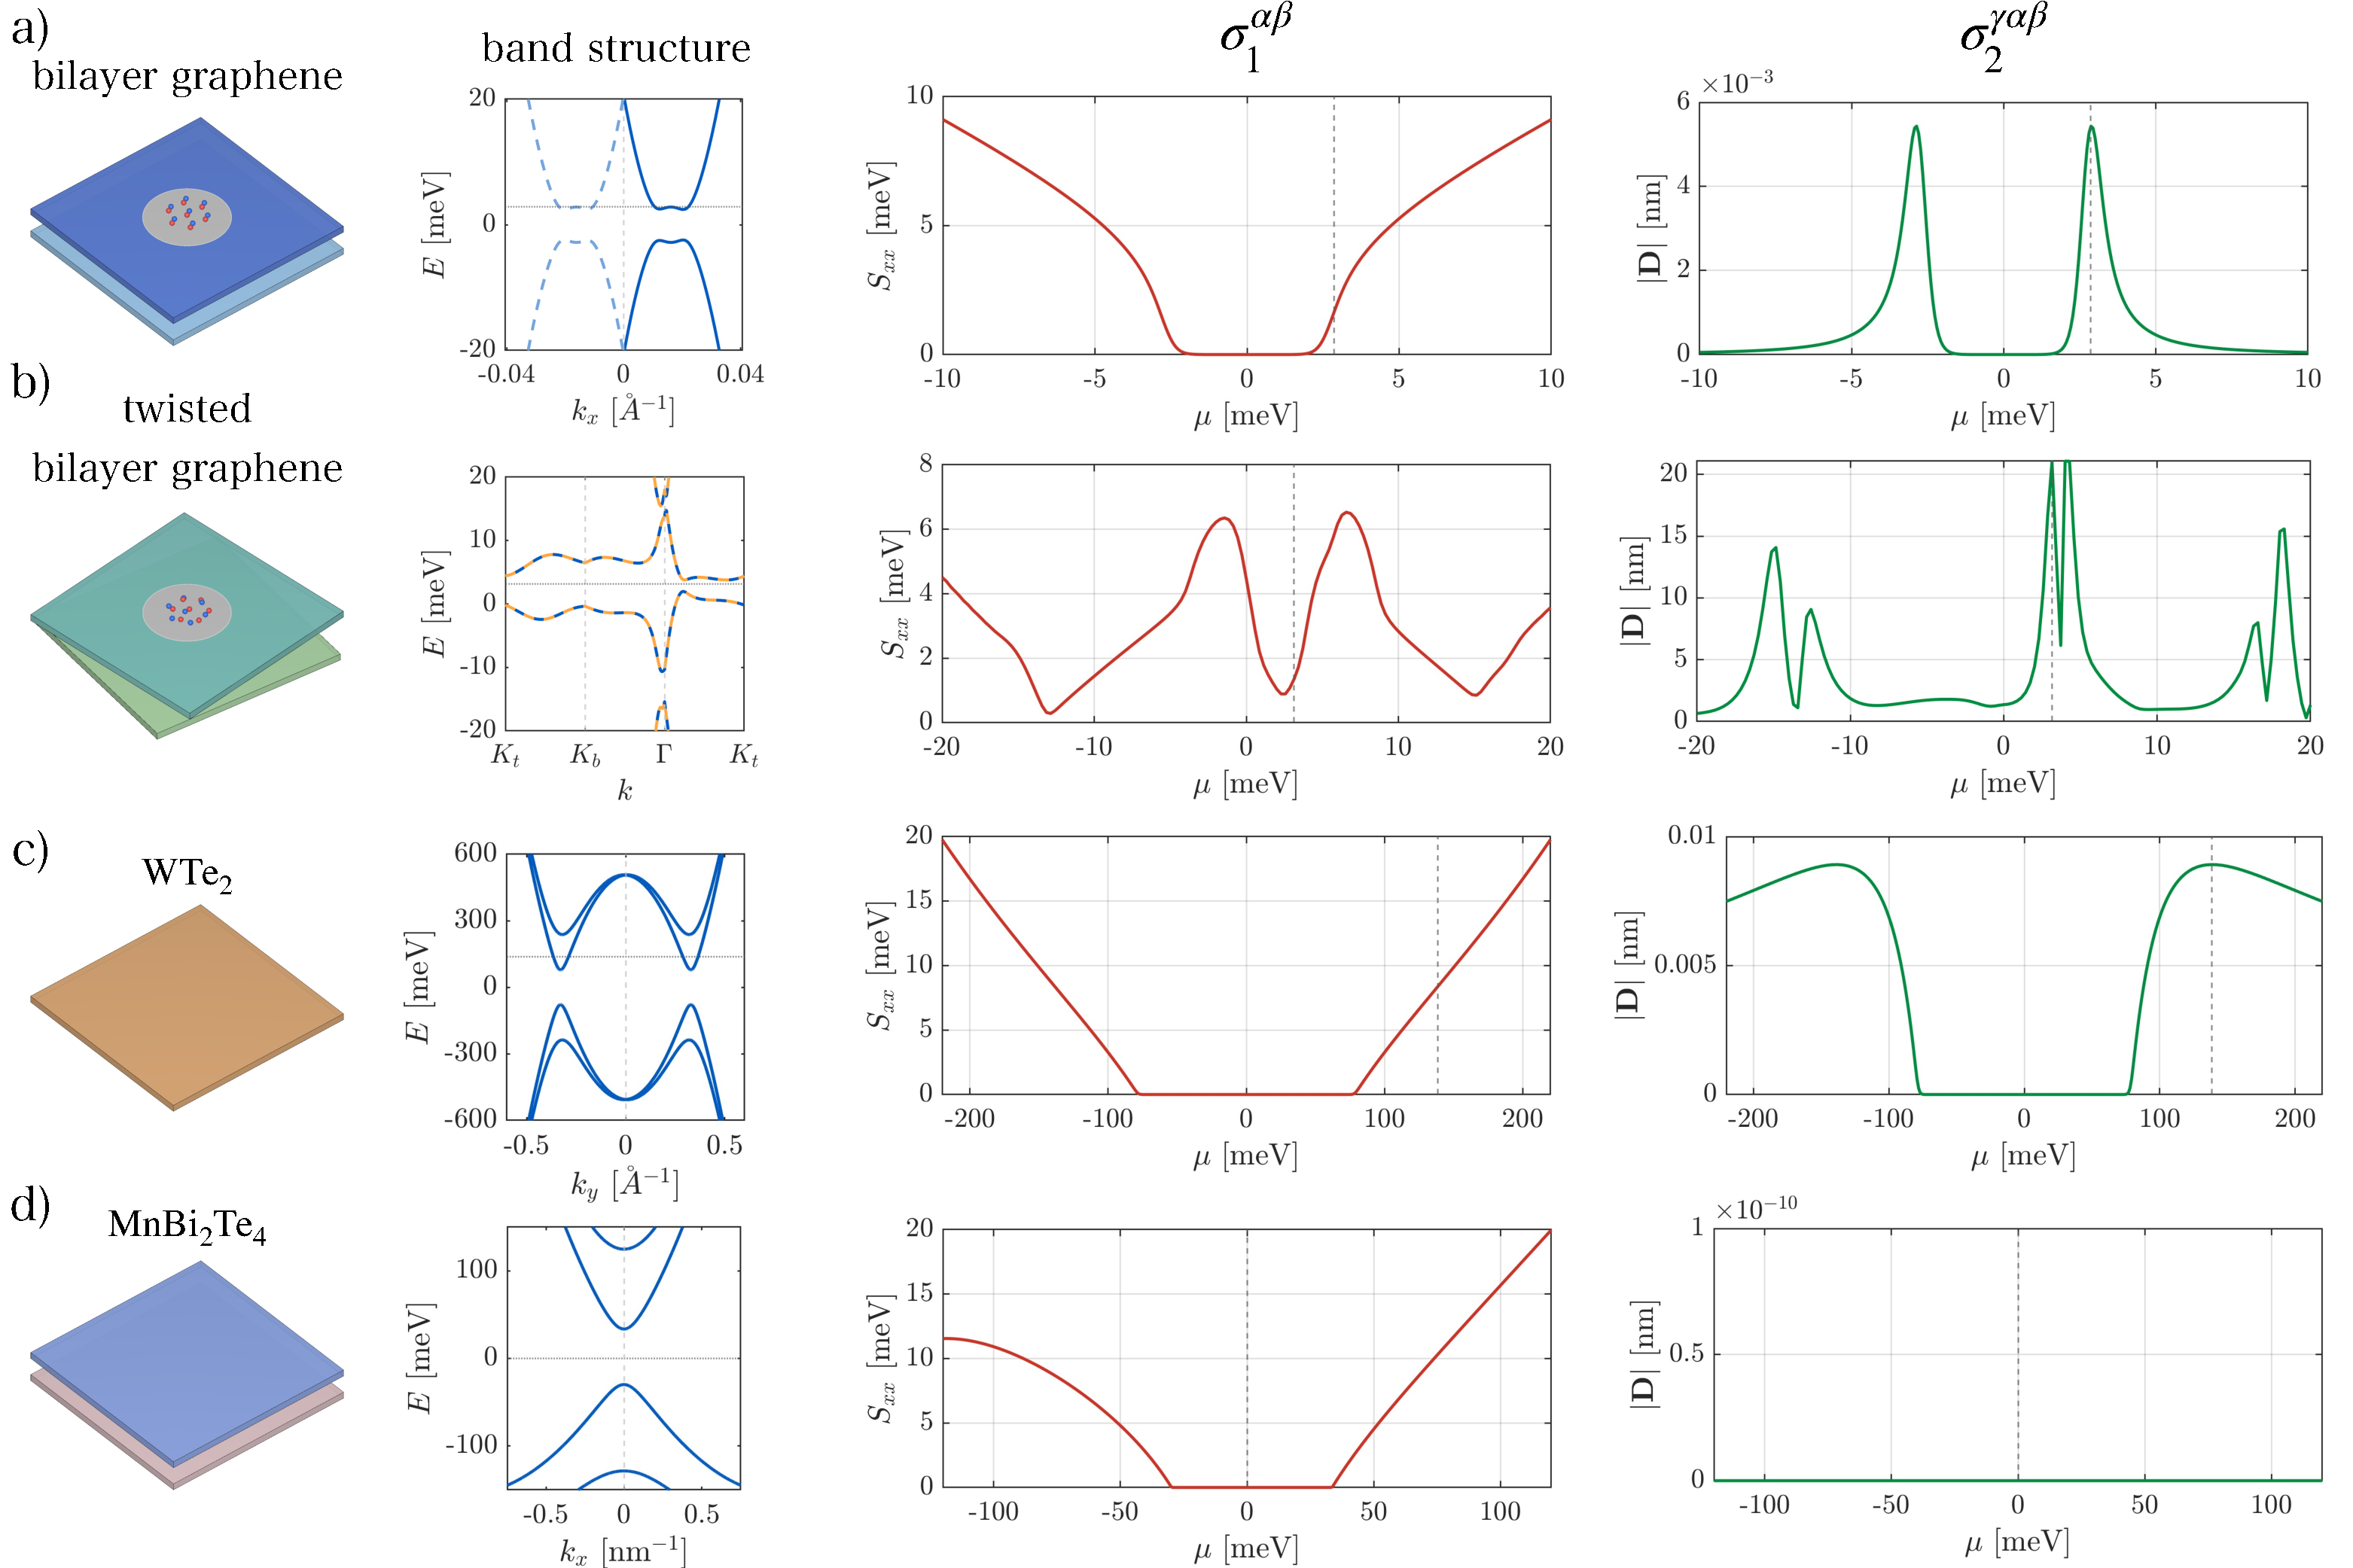
\includegraphics[width=0.95\textwidth]{NeuromorphicDevice3.pdf}
\caption{TBA.}
\label{fig3}
\end{figure*}

\subsection{Floquet reflection and transmission}

We model the 2D thin film as a conducting interface in the $x$--$y$ plane and consider a plane electromagnetic wave incident along the $z$ direction, i.e., at normal incidence. We denote the side containing the incident and reflected fields as medium 1, and the side containing the transmitted field as medium 2. The corresponding incident, reflected, and transmitted electric (magnetic) fields are denoted by $\mathbf E^i$ ($\mathbf H^i$), $\mathbf E^r$ ($\mathbf H^r$), and $\mathbf E^t$ ($\mathbf H^t$), respectively. Because a monochromatic drive can generate a multiharmonic response in the sample, the formalism is naturally generalized to include all harmonics.

We therefore expand the electromagnetic fields at the interface of the two media as
\begin{equation}
\mathbf E_n(\mathbf r,t)\hspace{-1mm}=\hspace{-1mm}\mathbf E_n e^{i(\mathbf k_n\cdot \mathbf r-\omega_n t)},~\mathbf H_n(\mathbf r,t)\hspace{-1mm}=\hspace{-1mm}\mathbf H_n e^{i(\mathbf k_n\cdot \mathbf r-\omega_n t)},
\end{equation}
where $\omega_n=n\Omega$, with $\Omega$ the frequency of the incident light, and $k_n/\omega_n = c\mu_0\varepsilon_0 = 1/c$. Since only the fundamental harmonic is incident, we have $\mathbf E_n^i \sim \delta_{n,1}$. Throughout, we use the Floquet-harmonic convention
\begin{equation}
F(t)=F(t+T)=\sum_{n=-\infty}^{\infty}F_n e^{-in\Omega t}.
\end{equation}
with $T = 2\pi/\Omega$ to be the period of the drive.

For normally incident radiation, the self-consistent Maxwell solution for the transmitted harmonic component takes the form (see \textbf{SI})
\begin{equation}
{\mathbf E_n^t+\frac{\mathbf j_n}{2c\epsilon_0}=\mathbf E_n^i,}
\end{equation}
where $\mathbf j_n$ is the $n$th harmonic of the induced surface current. This equation should be understood recursively, since higher harmonics of the transmitted field are generated by the nonlinear current response. In linear order, we obtain
\begin{equation}
\mathbf E_1^t=\left(1+\frac{\hat\sigma^1_{\Omega}}{2c\epsilon_0}\right)^{-1}\mathbf E_1^i.
\end{equation}

As expected, at linear order the transformation reduces to a standard linear mixing of the encoded features. At the same time, these 2D systems retain several tunable parameters, making them attractive for incorporation into a feedback-based learning loop. 

At second order, we find the media 2 emitted second harmonic becomes
\begin{equation}
{
\mathbf E_2^t=
-\frac{1}{2c\varepsilon_0}
\left(1+\frac{\hat\sigma^1_{2\Omega}}{2c\epsilon_0}\right)^{-1}
\hat\sigma^2_{\Omega,\Omega}:\mathbf E_1^t\mathbf E_1^t
}
\end{equation}
where the tensor contraction is defined as $\big[\hat\sigma^2_{\Omega,\Omega}:\mathbf E_1^t\mathbf E_1^t\big]_\gamma\equiv(\hat\sigma^2_{\Omega,\Omega})_{\gamma ij} E_{1,i}^t E_{1,j}^t.$ Importantly, the second-harmonic response already has a tensorial structure, in which the nonlinear Hall components naturally mix information from different Cartesian coordinates (see Fig. X).


\section{Dependence of transmittion properties on parameters}

\section{Device and computing primitives}


\section{Trainability and efficiency benchmarks of single layer graphene filter}

\section{Multi-layer device for deeper Kolmogorov-Arnold networks}
In this section we consider materials to be used for the photocurrent generation. A simple example is Option 1:
It is a minimal two-band model of a tilted massive Dirac cone, and the lattice version is its UV-regularized tight-binding analogue
\begin{equation}
H(\mathbf{k})=t_x k_x\,\mathbb{1}+v k_x \sigma_x+v k_y \sigma_y+m \sigma_z .
\end{equation}
Unfortunately Drude is UV log divergent. Better:
\begin{equation}
H(\mathbf{k})=t_x \sin k_x\,\mathbb{1}+v \sin k_x\,\sigma_x+v \sin k_y\,\sigma_y+\left(m+2-\cos k_x-\cos k_y\right)\sigma_z .
\end{equation}
with $a k_x,a k_y \in [-\pi, \pi]$, $v/vF =1$ ($v_F\sim 10^6$m/s$\sim 2.2$ eV), $m=1/4..1/40$ smaller - stronger BCD. 

\section{Conclusions and outlook}


\begin{acknowledgements}
D. O. O. acknowledges the support by Kavli Foundation.
\end{acknowledgements}


\bibliography{neuromorph_graphene_bib}

%\clearpage
%\input{supplement.tex}

\end{document}